\documentclass{article}
\usepackage{latexmldoc}

\title{\LaTeXML: a \LaTeX\ to \XML\ Converter; \emph{Preview}}
\author{Bruce R.~Miller}
\begin{document}
\maketitle
\section{Overview}
For many, \LaTeX\ is the prefered means for document authoring, particularly when
significant mathematical content is involved.
On the other hand, content-oriented \XML\ is an extremely useful storage format
allowing documents to be used, and reused, for a variety of purposes, not least, 
presentation on the Web.  Given the rough mismatch between the two,
particularly for mathematics, conversion  from \LaTeX\ to \XML\ is a bit tricky.
Faced with this situation, and the lack of other suitable tools at that time,
the \URL[Digital Library of Mathematical Functions]{http://dlmf.nist.gov}
proceeded to develop thier own tool, \LaTeXML, to fill this need.
This document describes a \emph{preview} release of \LaTeXML.

The idealistic goals of \LaTeXML\ are:
\begin{itemize}
\item Faithful emulation of TeX's behaviour.
\item Easily extensible.
\item Lossless; preserving both semantic and presentation cues.
\item Uses abstract \LaTeX-like, extensible, document type.
\item Determine the semantics of mathematical content\\
    (Content \MathML, \emph{Good} Presentation \MathML, eventually \OpenMath).
\end{itemize}

As these goals are not entirely practical, or somewhat contradictory,
they are implicitly modified by ``as much as possible.''
Completely mimicing \TeX's behaviour would seem to require the sneakiest modifications
to \TeX, itself.  `Ease of use,' of course, is in the eye of the beholder.
Few documents are likely to have completely unambiguous mathematics markup; 
human understanding of both the topic and the surrounding text is needed to
properly interpret any particular mathematical fragment.
Thus, we expect that document-specific declarations or tuning to be necessary
to faithfully convert mathematical documents, rather than presuming to
provide a `turn-key' solution. At the same time, we would encourage
a more content-oriented mathematical markup style, than a presentation-oriented style.

\medskip
This document continues with an overview of the usage of \LaTeXML (\S\ref{sec:usage})
and it's architecture (\S\ref{sec:architecture}).   
In \S\ref{sec:packages}, an overview of customizing \LaTeXML\ is given.
How mathematics is converted to content-oriented forms is discussed in \S\ref{sec:math}.
Finally, Appendix \ref{app:architecture} gives slightly more details about the architecture,
and Appendix \ref{app:todo} lists the main problem areas and unfinished features.
In general, for more detail, you should see the perl documentation of various
\LaTeXML\ Packages, or the source code and examples, themselves.

\section{Using \LaTeXML}\label{sec:usage}
The basic conversion to \XML\ (using the \LaTeXML\ DTD, by default) is carried out
by the command:
\begin{quote}
 \cmd{latexml \textit{options} document.tex > document.xml}
\end{quote}
The more useful command options are
\begin{description}
\item[\cmd{--path}=\textit{dir}] Adds \textit{dir} to the list of paths used to search
  for files (packages, style files, etc). Similar to \texttt{TEXINPUTS}.
\item[\cmd{--preload}=\textit{package}] Loads a Package before processing.  This may
  be useful to load a package that would not otherwise be automatically loaded 
  due to a \verb|\usepackage| or similar command.  See \S\ref{sec:packages}.
\end{description}
See \cmd{latexml --help} for other options that may be useful for debugging.

Additional transformations, particularly the parsing of mathematical content, are carried out
by the postprocessor \cmd{latexmlpost}:
\begin{quote}
\cmd{latexmlpost \textit{options} document.xml}
\end{quote}
where the options are:
\begin{description}
\item[\cmd{--stylesheet=\textit{stylesheet}}] requests an \texttt{XSLT} transformation of
    the \XML\  using the given stylesheet.
\item[\cmd{--format=(html|xhtml)}]  Specifies the format for conversion. Default
    is to leave as \XML.
\item[\cmd{--destination=\textit{file}}]  Specifies the file to write the output.
    If the file has either an html or xhtml extension, that format is assumed.
\item[\cmd{--source=\textit{dir}}] Some postprocessing (eg. transforming graphics files)
     may need access to the directory  where the original \TeX\ file resided 
     (if it isn't the current working directory).
\item[\cmd{--verbose}] Increases the amount of messages about the progress of processing.
\item[\cmd{--help}] Prints a brief description of the command and options.
\end{description}
Transforming to html format involves parsing math formula and converting them to Presentation MathML,
transforming tables into an HTML consistent format, converting graphics files and applying 
an XSLT transformation.
Transforming to html format is similar, but math formula are converted to images.
If no format is specified, only math parsing and conversion is done.

\section{Architecture}\label{sec:architecture}
Like \TeX, \LaTeXML\ is data-driven: the text and control sequences\footnote{\TeX's name
for the backslashed commands; ie.~macros, primitives and so forth}
in the source file (and packages used, being simply collections of macros)
direct the processing.
You exert control over the processing, and customize it, by 
the \emph{implementation} of the control sequences (or packages).
That, or by postprocessing --- all the heavy-lifting that implements parsing 
of mathematics is carried out in postprocessing; See \S\ref{sec:math}.


\begin{figure}[tb]
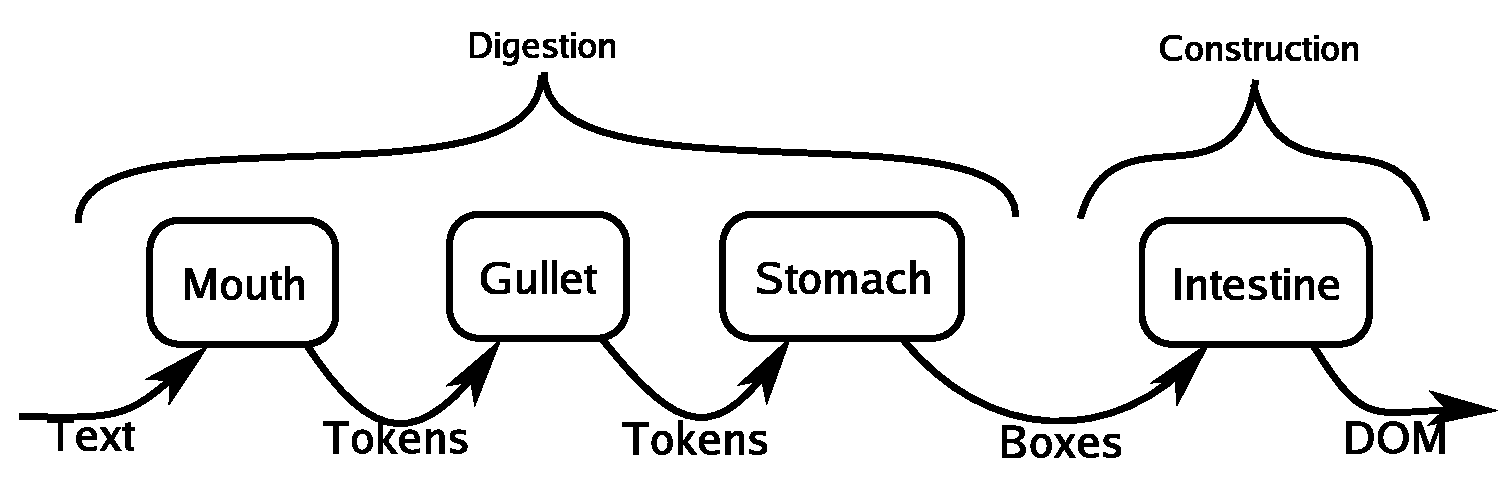
\includegraphics[width=\columnwidth]{dataflow}
\caption{Flow of data through \LaTeXML's digestive tract.\label{fig:dataflow}}
\end{figure}
Roughly, \TeX's digestive tract is emulated as follows; See Figure \ref{fig:dataflow}.
The processing is broken into two phases; digestion and construction.
The \pkg{Stomach}  maintains the current state of processing during digestion;
it sets up a chain consisting of a \pkg{Mouth} (to convert characters from the file into \pkg{Token}'s) 
and a \pkg{Gullet} (to read \pkg{Token}'s from that \pkg{Mouth}, expanding any \pkg{Macro} or
\pkg{Expandable} tokens).
It then reads \pkg{Token}'s from the \pkg{Gullet} and digests them
(executing \pkg{Primitive}'s and converting \pkg{Constructor} tokens to \pkg{Whatsit}'s).
These three components operate in \emph{pull mode}, each pulling data from the previous.
The \pkg{Stomach} digests all available input, converting the \pkg{Token}'s into
a recursive \pkg{List} of \pkg{Box}'s, \pkg{List}'s, and \pkg{Whatsit}'s.

Document construction is carried out by the \pkg{Intestine}, which recursively traverses 
the \pkg{List} constructs a \pkg{DOM}, representing the \XML\ document tree.
The key features for generating \XML, are the control sequences that we
call `constructors', and our extension of the concept of a \pkg{Whatsit} that generate arbitrary
\XML\ fragments.

This process is described in slightly more detail in Appendix \ref{app:architecture}, but
see the perl documentation \cmd{perldoc} for the modules for the APIs, and, ultimately,
the source for full details.


\section{Packages: Implementing Control Sequences}\label{sec:packages}
The processsing of the \LaTeX\ document and it's  conversion into \XML\ is affected
by the definitions of control sequences, either as macros, primitives or constructors, 
and other declarations specifying the document type, properties of \XML\ tags, ligatures, \ldots.
These definitions and declarations are typically contained in `packages' which provide
the implementation of \LaTeX\ classes and packages.  For example, the \LaTeX\ directive
\verb|\usepackage{foo}| would cause \LaTeXML\ to load the file \code{foo.ltxml}.
This file would be sought in any of the directories in perl's \verb|@INC| list (typically
including the current directory), or in a \verb|LaTeXML/Package| subdirectory of any of 
those directories.

The following packages are loaded before processing the document \textit{jobname}\texttt{.tex}:
first the \pkg{TeX} package is loaded, then any packages named in
the \verb|--preload| option is loaded, then a file \textit{jobname}\texttt{.latexml}, if 
present, is loaded, providing for document-specific declarations.
Document processing then commences; by default assuming that the document is plain \TeX.
However, if a \verb|\documentclass| directive encountered, the \pkg{LaTeX} package, as well
as a package for the named class are loaded.

The facilities available for implementing packages is described in \perldoc{LaTeXML::Package}.

\section{Mathematics}\label{sec:math}
The mathematical material is parsed into a content-oriented representation following
the usual steps: lexical scanning, grammar-based parsing and (eventually) type-analysis, but
with a few twists. As \LaTeXML\ constructs the initial document, the mathematical material
is converted mainly into a sequence of lexical tokens (\tag{XMTok}), possibly carrying extra information
such as name, partOfSpeech, font, style, etc.  The exceptions are where 
the mathematical structure is clear from the markup itself, such as \verb|\frac| or sub- and
superscripts, where an application (\tag{XMApp}) is constructed.  The substructures will 
typically be wrapped in either an \tag{XMArg} or \tag{XMWrap} element; the former for when 
the substructure should also be parsed as a complete subexpression, the latter when it is 
expected to be sloppy and may not be sensibly parsed (explain this!).
Thus we speak of \LaTeXML\ as being a \emph{structure preserving lexer}.  

The parser, invoked by the postprocessor, works only with the top-level lists of lexical tokens,
or with those sublists contained in an \tag{XMArg}.  The grammar works primarily through
the name and partOfSpeech (\code{POS}).  The name is given by an attribute, or the content if it is
the same.  The partOfSpeech (things like ID, FUNCTION, OPERATOR, OPEN, \ldots) is also given
by an attribute, or, if not present, the name is looked up in a document-specific
dictionary (\textit{jobname}\texttt{.dict}), or in a default dictionary.

Additional exceptions that need fuller explanation are: 
(1) \pkg{Constructors} may wish to create a dual object (\tag{XMDual}) whose children are 
the semantic and presentational forms.
(2) Spacing and similar markup generates \tag{XMHint} elements, which are currently ignored
during parsing, but probably shouldn't.

\appendix
\section{Architectural Details}\label{app:architecture}
\subsection{Tokenization}

\paragraph{\lpkg{Mouth}}
Given a string or file, a \pkg{Mouth} tokenizes the input text according to
the current category codes in the \pkg{Stomach}. Category codes distinguish classes of characters
such as plain characters, control sequences,  active characters and \TeX's special characters  
for grouping,  sub- and super-script and math mode.  The main method is \method{readToken}, which
returns the next \pkg{Token} from the input.
(See \perldoc{LaTeXML::Mouth})

\paragraph{\lpkg{Token}, \lpkg{Tokens}} These packages represent a Token (a pair containing a character
or string and the category code) and a list of \pkg{Token}'s.  The latter responds to the same
interface as \pkg{Mouth}, so it can also be read from.
(See \perldoc{LaTeXML::Token})

\subsection{Expansion}

\paragraph{\lpkg{Gullet}}
The \pkg{Gullet} reads \pkg{Token}'s from the \pkg{Mouth}, possibly expanding them.
The main methods are \method{readToken} and  \method{readXToken}.
The latter returns the next unexpandable \pkg{Token} from the input;
if the token's current meaning in the \pkg{Stomach} is a \pkg{Macro} or \pkg{Expandable},
it is expanded and its expansion is replaced in the input before retrying.
(See \perldoc{LaTeXML::Gullet})

\paragraph{\lpkg{Expandable}, \lpkg{Macro}} Instances of these packages (subclasses of \lpkg{Definition})
represent the expansions of control sequences. \pkg{Expandible} typically are used for
conditionals (like \verb|\if|, \verb|\ifx|, \ldots) and built-in control sequences that expand 
into sequences of \pkg{Token}'s (such as \verb|\jobname|).  \pkg{Macro} are typically used
to replace the control sequence with a list of \pkg{Token}'s.
(See \perldoc{LaTeXML::Definition})

\subsection{Digestion}
\paragraph{\lpkg{Stomach}}
The \pkg{Stomach} maintains global state during digestion and carries out the digestion of \pkg{Token}'s.
The top-level method \method{readAndDigestFile(\$file)} sets up the initial state and stack, 
pre-loads packages (at least \code{TeX}), and then digests all available input, 
returning the digested \pkg{List}.

The \pkg{Mouth} and \pkg{Gullet} refer to the \pkg{Stomach} to set or access the mode, various values and
definitions (The variable \verb|$LaTeXML::STOMACH| is bound (\code{local}) to current 
\pkg{Stomach} object, so that it can be accessed from various odd places).
To mimic \TeX's binding of definitions and values scoped by grouping, 
the \pkg{Stomach} maintains a \emph{stack}, with each stack frame corresponding to a \TeX\ group.
Look-ups generally proceed by searching the stack for a frame that contains a value for the quantity
in question.  (See \perldoc{LaTeXML::Stomach})

Basically, there are four cases when digesting a \pkg{Token}:
 \begin{itemize}
  \item Plain characters are simply converted to a \pkg{Box} (or \pkg{MathBox} in math mode), 
   recording the current \pkg{Font}.
  \item Control sequences representing a \pkg{Primitive} are executed.  This is typically
   done for side effect (changing the state in the \pkg{Stomach}), although they may also
   contribute \pkg{List}'s, \pkg{Box}'s or \pkg{Whatsit}'s.
   As with \pkg{Macro}'s, any arguments to the \pkg{Primitive} are read from the \pkg{Gullet}.
  \item Grouping (or environment bodies) are collected into a \pkg{List}
   (or \pkg{MathList} in math mode).
  \item A special class of control sequence, called a \pkg{Constructor} produces a 
   \pkg{Whatsit} which remembers the control sequence and arguments that
   created it, and defines it's own translation into \XML\ elements, attributes and data.
   Arguments to a \pkg{Constructor} are read from the \pkg{Gullet} and also digested.
 \end{itemize}
Finally, \pkg{Filter}'s are applied to the resulting \pkg{List}'s (see below).

\paragraph{\lpkg{Box}, \pkg{MathBox}, \pkg{List}, \pkg{MathList}, \pkg{Whatsit}} Instances of
these classes represent the digested objects: boxes being characters; lists being sequences
of digested objects; whatsits representing some sort of document fragment.
Note that, currently, Although \verb|\par| tends to do the `right thing', there 
is no real notion of horizontal or vertical mode.
(See \perldoc{LaTeXML::Box})

\paragraph{\lpkg{Primitive},\lpkg{Constructor}} These classes of \pkg{Definitions} are carried out
(at least partly) in the \pkg{Stomach}. They may have before and after daemons; little bits
of code that affect the state.  A \pkg{Primitive} is carried out for only side-effect,
but a \pkg{Constructor} generates a \pkg{Whatsit} that survives to the \pkg{Intestine}.
(See \perldoc{LaTeXML::Definition}).


\paragraph{\pkg{Filter}} Filters are roughly a generalization of ligatures. They are matched
against sequences of digested items during digestion; if they pattern is matched, it is substituted
by the replacement.  They are currently defined for the kinds of substitutions that would
make sense for \XML; namely repeated characters like \texttt{-} or \texttt{`} are replaced by 
the appropriate unicode. Also, in math, patterns of digits or letters (in non-mathitalic fonts) 
are combined as one would expect.  On the other hand, ligatures like \texttt{ffi} do not
really seem appropriate here --- or do they? --- they would be easily implemented, but
they might adversely affect search.

\paragraph{\lpkg{Font}} A representation of font, size and color.

\subsection{Construction}
\subsubsection{\lpkg{Intestine}}
The \pkg{Intestine} traverses the recursive \pkg{List} of \pkg{List}'s, 
\pkg{Box}'s and \pkg{Whatsit}'s, constructing a Document Object (\pkg{DOM}),
according to the current \pkg{Model}.  Generally, a \pkg{Box} gives rise to text data, whereas
a \pkg{Whatsit} describes a document fragment (consisting of elements, thier attributes and or content).
At each insertion, the \pkg{Model} is consulted to determine if the insertion is allowed at the
current point, or if intermediate elements may need to be opened or closed.
This allows the document structure of sections and paragraphs to be automatically
constructed, for example, even though \LaTeX\ doesn't explicitly close \verb|\section|,
nor open \verb|\par|.
(See \perldoc{LaTeXML::Intestine},  \perldoc{LaTeXML::DOM},  \perldoc{LaTeXML::Model}).


\section{Issues and ToDo}\label{app:todo}
Lots\ldots!
\begin{itemize}
\item Lots of useful \LaTeX\ packages have not been implemented, and those
  that are aren't necessarily complete.
\item \TeX\ boxes aren't really complete, and in particular things like \verb|\ht0|
  don't work.
\item Possibly useful to override (pre-override?) a macro defined in the source file;
  that is, define it and silently ignore the definition given in the source.
\item \ldots um, \ldots \emph{documentation}!
\end{itemize}
\end{document}
